\newpage
\chapter{Experiments}
\label{sec:experiments}
\hl{SECTION UNDER CONSTRUCTION}\\
The experiments with the Evo-RoleMiner shall provide information, which is not given in Saenko \& Kotenko \cite{saenko2012design}. In particular how parameters can be set and how the objectives of the role models evolve and impact other objectives. Afterwards the MOEA Evo-RoleMiner$M$ is tested and compared to EA EvoRoleMiner. Also the EvoRoleMiner and EvoRoleMiner$M$ are tested on datasets commonly used in role mining research.

This chapter describes the setup of the experiments executed. First the data sets used in the experiments are described. Then the setup and the results of the experiments are introduced. The experiments have been divided into several steps, where the results of one experiment lead to the setup of the experiments after.

In the first experiment  single objective measures introduced in section \ref{sec:optimizationCompleteness}, \ref{sec:optimizationComplexity} and \ref{sec:optimizationComprehension} are set as fitness function in the Evo-RoleMiner. This experiment set was executed to validate the implementation of the objective functions, which are combined at a later stage, and to analyse the impact of these objectives to each other. In the second and third set of experiments the actual fitness functions for the Basic-RMP and Min-Edge-RMP (see section \ref{sec:fitnessFunctions}) are tested in the Evo-RoleMiner. In a later set of experiments the Evo-RoleMiner$M$ is tested as well as the Interpretability measure (see section \ref{sec:classifierRule}) and constraints.

All experiments have been executed ten times and started with a random start-population. The experiments have been executed mainly on the healthcare dataset (see Figure \ref{fig:healthcare}) and on a synthetic dataset generated by the data generator (see Figure \ref{fig:dataset1}).

\section{Data Sets}
\subsection{Real Datasets}
In many research papers the same datasets are used for performance evaluation of role mining algorithms. Table \ref{tab:realDatasets} lists some of these data sets and their components. The authors of \cite{Ene} obtained these datasets from Cisco firewalls and the Lotus Domino server of the Hewlett Packard (HP) networks. The healthcare dataset was collected from the US Veteran’s Administration.

\begin{table}[H]
    \centering
    \begin{tabular}{|l|l|l|l|}
        \hline
        \rowcolor{myGray} 
        \textbf{Dataset} & \textbf{$|U|$} & \textbf{$|P|$} & \textbf{$|UPA|$} \\ \hline
        healthcare       & 46             & 46                   & 1486                                 \\ \hline
        domino           & 79             & 231                  & 730                                  \\ \hline
        emea             & 35             & 3046                 & 7220                                 \\ \hline
        apj              & 2044           & 1146                 & 6841                                 \\ \hline
        firewall-1       & 365            & 709                  & 31951                                \\ \hline
        firewall-2       & 325            & 590                  & 36428                                \\ \hline
        americas-small   & 3477           & 1587                 & 105205                               \\ \hline
    \end{tabular}
    \caption{Real Datasets used in Role Mining research. The table lists the amount of users, permissions and user-permission assignments in each dataset.}
    \label{tab:realDatasets}
\end{table}

\subsection{Synthetic Datasets}
The real dataset commonly used in Role Mining research (see Table \ref{tab:realDatasets}) do not provide user attribute information. Only Xu \& Stolter\cite{Xu} are generating synthetic attribute information on the given datasets. Also the data generators for synthetic datasets for role mining are only providing user-permission assignment information, but no user attribute information, e.g. in Vaidya et al.\cite{Vaidya:2006:RMR:1180405.1180424}.

In order to test smaller datasets with user attribute information where an optimal solution is known, a new synthetic data generator has been created for this thesis. The data generator allows to adjust, amongst other configurations, the dimensions of users and permissions, the density of user-permission assignments and user attribute information. The data generator is based on a reversed role-engineering process and generates users, roles, user attribute rules for the roles, user-role matrix, role-permission matrix, user-permission matrix and a user-permission matrix with noise. A more detailed description of the data generator can be read in the Appendix \ref{sec:A_dataGenerator}.

Two datasets have been generated with the data generator in order to execute experiments with fitness functions $F_{basic\_INT}^{min}$ \eqref{eq:FBasicMin_INT} and $F_{edge\_INT}^{min}$ \eqref{eq:FEdgeMin_INT}. The synthetic datasets are listed in table \ref{tab:syntheticDatasets}.

\begin{table}[H]
    \centering
    \begin{tabular}{|l|c|c|c|c|}
        \hline
        \rowcolor{myGray} 
        \textbf{Dataset} & \textbf{$|U|$} & \textbf{$|P|$} & \textbf{$|UPA|$} & \textbf{$|R|$}\\ \hline
        1       & 10    & 10   & 42    & 4\\ \hline
        2       & 50    & 50   & 620   & 15\\ \hline
    \end{tabular}
    \caption{Synthetic Datasets}
    \label{tab:syntheticDatasets}
\end{table}

A visualization of synthetic dataset 1 and the healthcare dataset can be seen in Figure \ref{fig:dataset1} and \ref{fig:healthcare}. Visualizations of the other real datasets can be seen in the Appendix \ref{sec:A_real_datasets}. Detailed information about the generated synthetic datasets can be found in Apendix \ref{sec:A_syn_datasets}.

\begin{figure}[H]
    \centering
    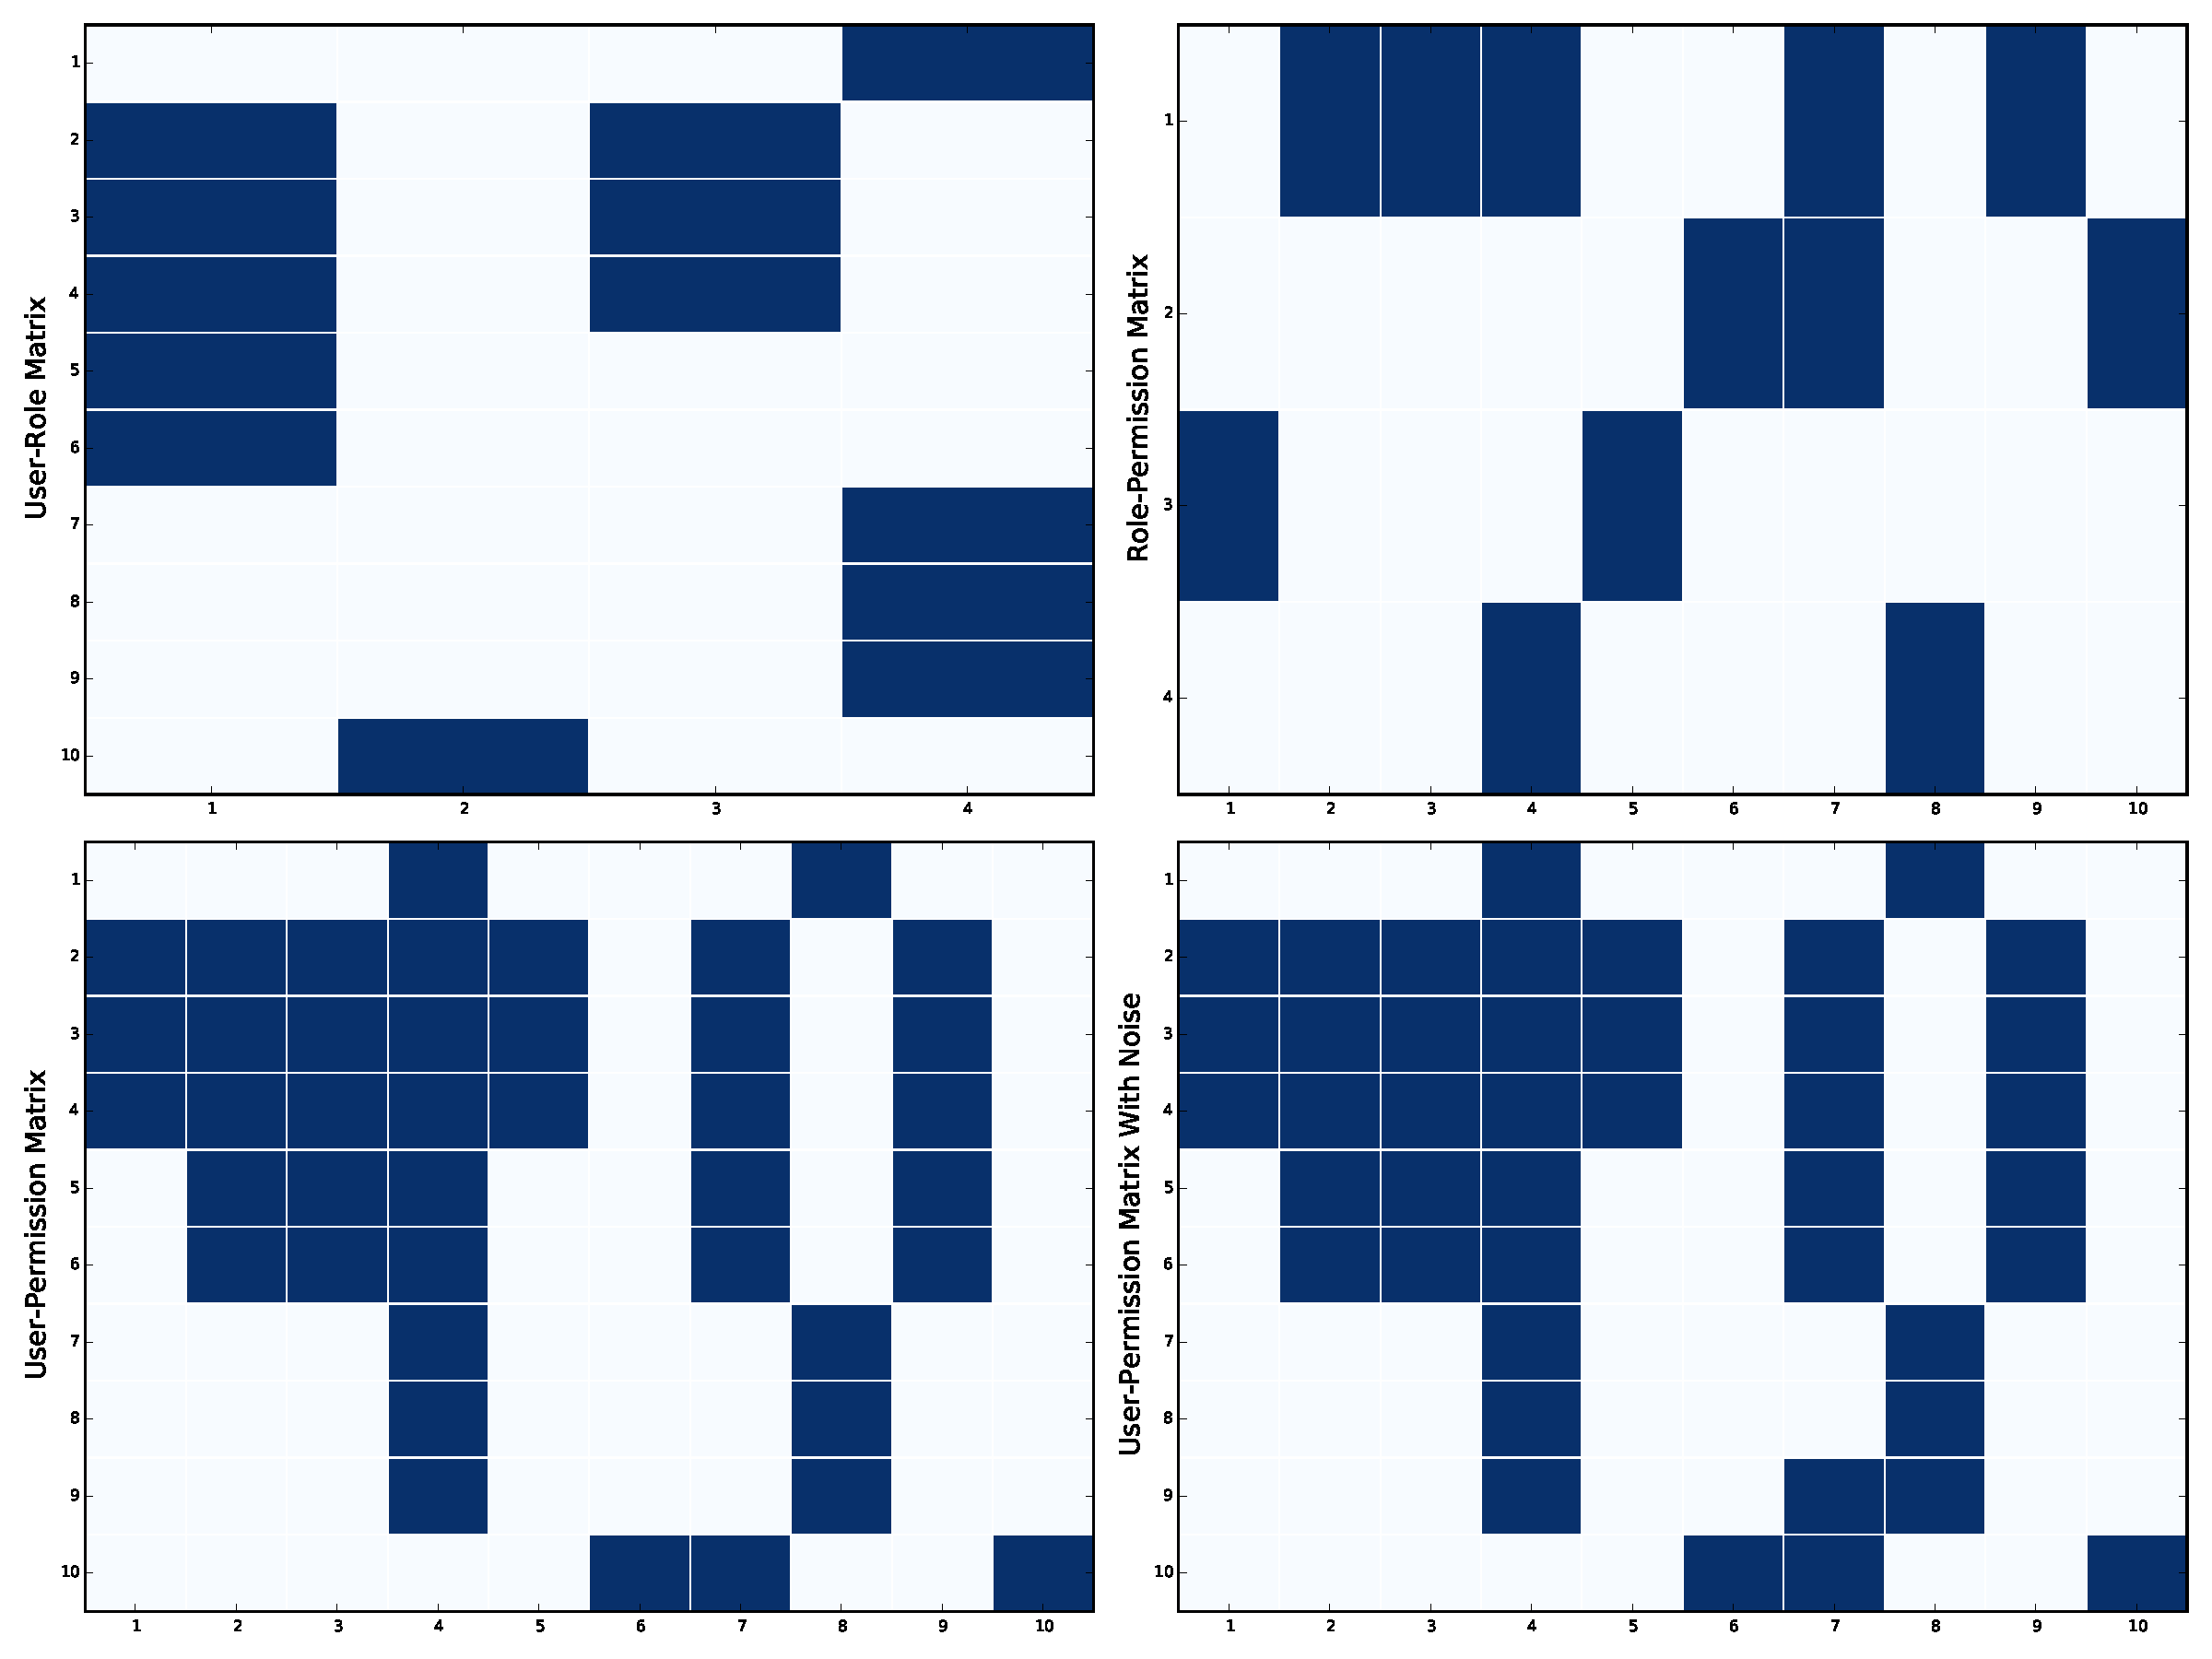
\includegraphics[width=0.7\textwidth]{dataset1}
    \caption{DATASET 1: Role model of synthetic dataset 1 including User-Permission Matrix. From u.l. to l.r.: User-Role Matrix (Rows: Users, Columns: Roles), Role-Permission Matrix (Rows: Roles, Columns: Permissions), Resulting User-Permission Matrix (Rows: Users, Columns: Permissions), User-Permission Matrix with Noise (Rows: Users, Columns: Permissions)}
    \label{fig:dataset1}
\end{figure}

\begin{figure}[H]
    \centering
    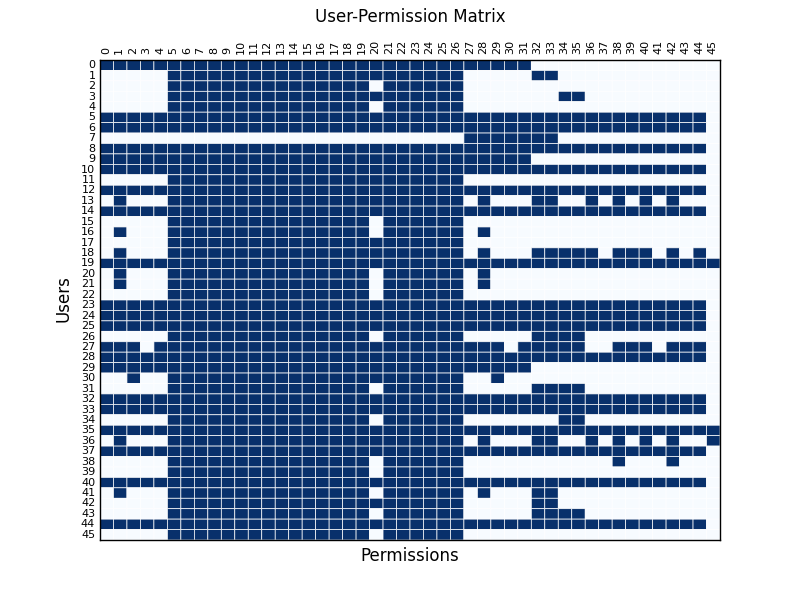
\includegraphics[width=0.7\textwidth]{healthcare}
    \caption{HEALTHCARE DATASET: User-Permission Matrix}
    \label{fig:healthcare}
\end{figure}

\import{chapters/}{10_Experiment1.tex}
\import{chapters/}{10_Experiment2.tex}
\import{chapters/}{10_Experiment3.tex}
\import{chapters/}{10_Experiment4.tex}
\import{chapters/}{10_Experiment5.tex}
\import{chapters/}{10_Experiment6.tex}
\import{chapters/}{10_Experiment7.tex}

\section{Experiments with Co-Evolution}
\hl{SECTION UNDER CONSTRUCTION}\\
\subsection{Setup}
\subsection{Measures}
